\documentclass[]{article}
\usepackage{datetime}
\usepackage{color,array,graphics}
\usepackage{enumerate}
\usepackage{mathtools}
\usepackage{amsmath}
\usepackage{amssymb}
\usepackage{bbm}
\usepackage{graphicx}
\usepackage{pgfplots}
\usepackage {tikz}

\addtolength{\oddsidemargin}{-.875in}
\addtolength{\evensidemargin}{-.875in}
\addtolength{\textwidth}{1.75in}

\addtolength{\topmargin}{-.875in}
\addtolength{\textheight}{1.75in}
\voffset0.0in

\def\OR{\vee}
\def\AND{\wedge}
\def\imp{\rightarrow}
\def\math#1{$#1$}
\def\mand#1{$$#1$$}
\def\mld#1{\begin{equation}#1\end{equation}}
\def\eqar#1{\begin{eqnarray}#1\end{eqnarray}}
\def\eqan#1{\begin{eqnarray*}#1\end{eqnarray*}}
\def\cl#1{{\cal #1}}

\newcommand\tab[1][0.62cm]{\hspace*{#1}}

\DeclareMathAlphabet{\mathpzc}{OT1}{pzc}{m}{it}
\DeclareSymbolFont{AMSb}{U}{msb}{m}{n}
\DeclareMathSymbol{\N}{\mathbin}{AMSb}{"4E}
\DeclareMathSymbol{\Z}{\mathbin}{AMSb}{"5A}
\DeclareMathSymbol{\R}{\mathbin}{AMSb}{"52}
\DeclareMathSymbol{\Q}{\mathbin}{AMSb}{"51}
\DeclareMathSymbol{\I}{\mathbin}{AMSb}{"49}
\DeclareMathSymbol{\C}{\mathbin}{AMSb}{"43}



\begin{document}
Alexander Garcia

6 October 2016

661534755

\centerline{\bf \Large Assignment 5}

\medskip

\noindent (1) (a) \textbf{A}. Each node in the binary tree has at most one parent, making option III incorrect.

(b) \textbf{A}. In a full binary tree, each node that is not a leaf has exactly two children, making options I and IV incomplete. \\

\noindent (2) $2200^{2200} \equiv x$ (mod 3)

$2200 \equiv ?$ (mod 3)

$2200 \equiv 1$ (mod 3)

$2200^{2200} \equiv 1^{2200}$ (mod 3)

\textbf{B} \\

\noindent (3) \textbf{D}. There are three paths that result in 15ms delays.

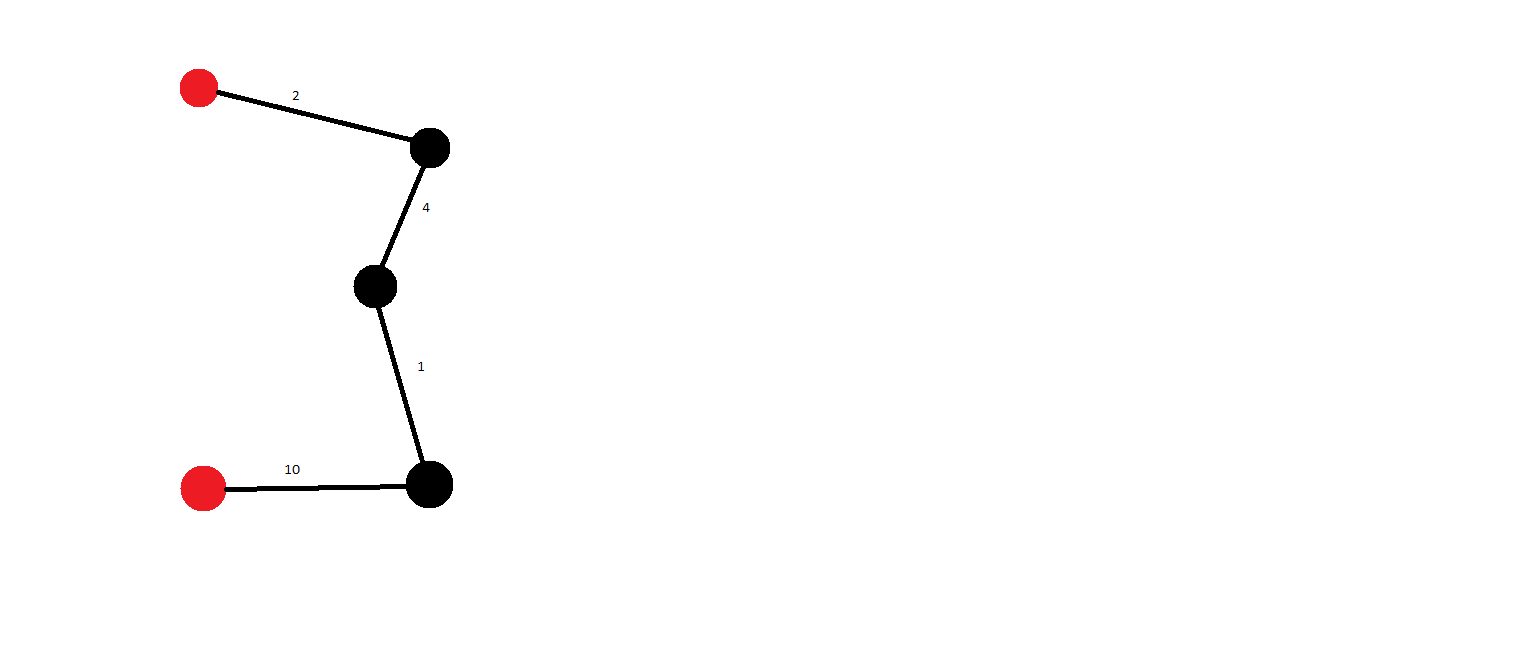
\includegraphics[scale=0.2]{path1.png}
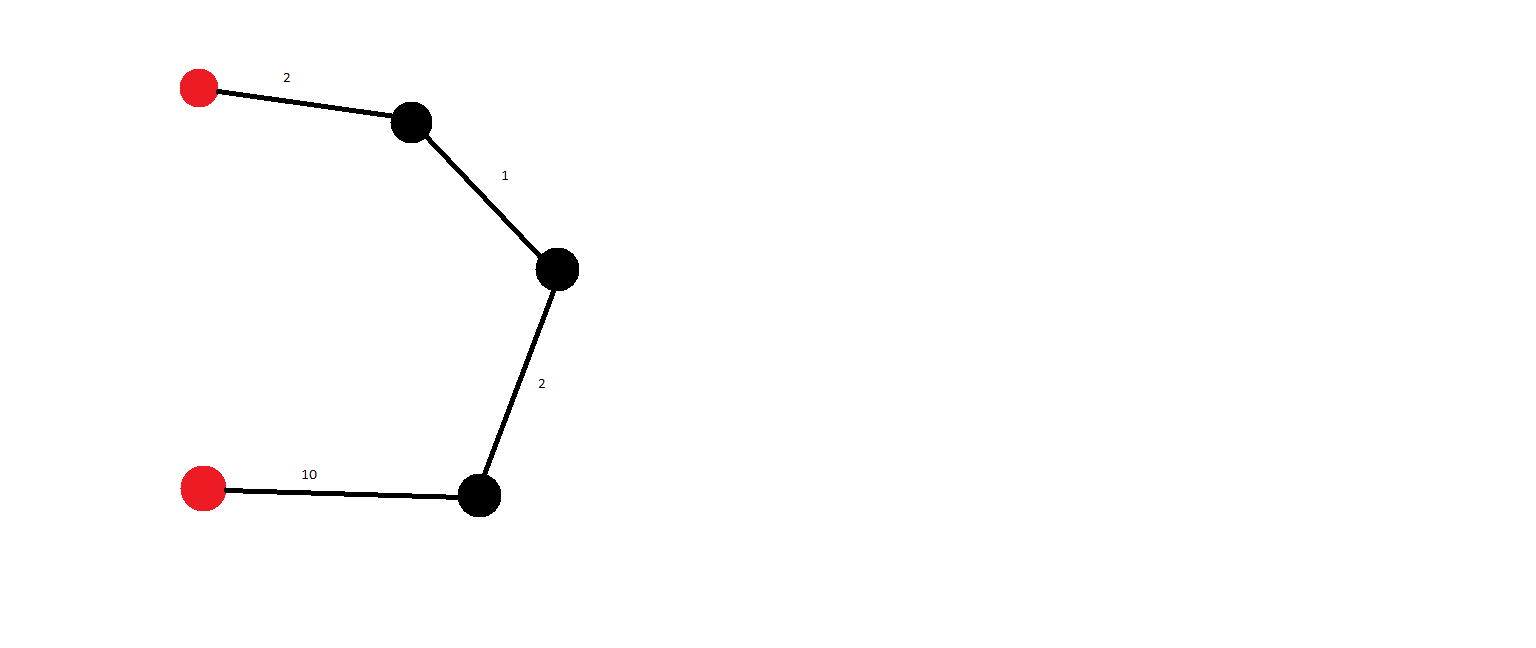
\includegraphics[scale=0.2]{path2.png}
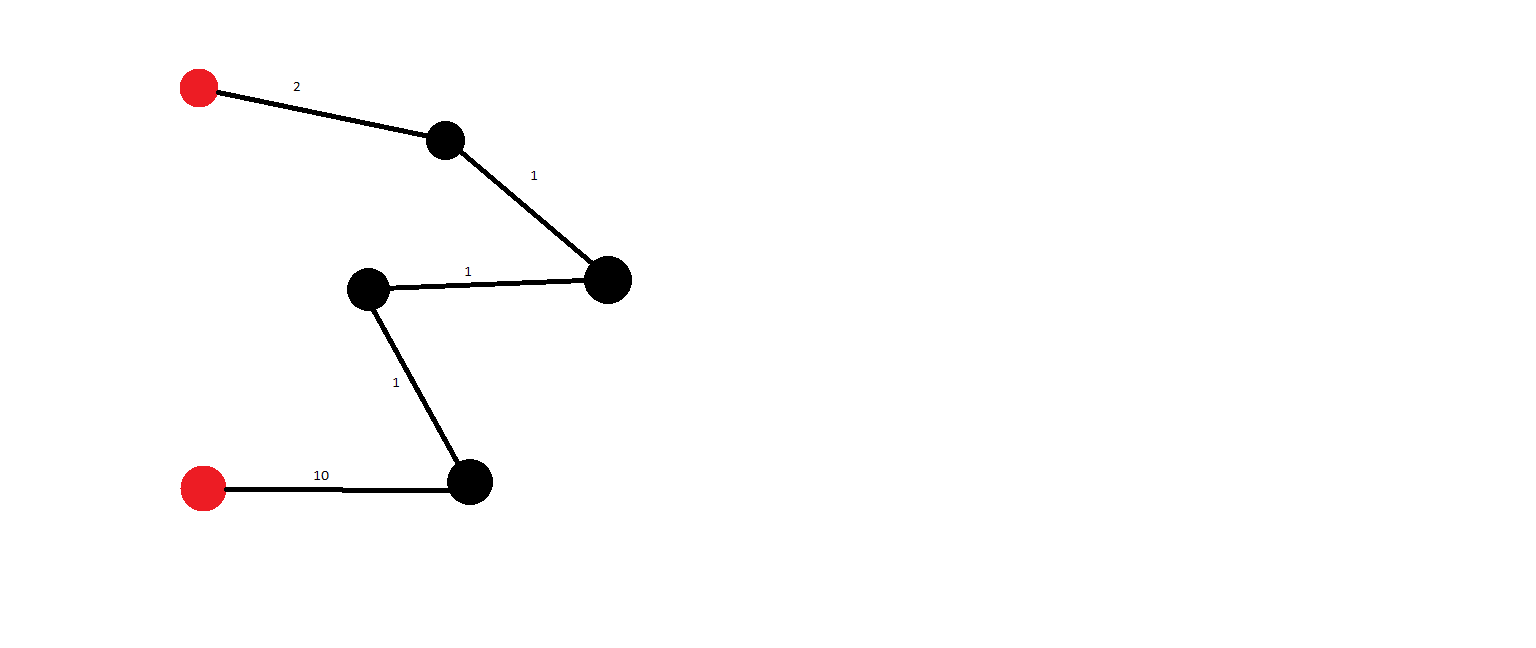
\includegraphics[scale=0.2]{path3.png}\\

\noindent (4)

\begin{tikzpicture}
\begin{axis}[
	axis lines=center,
	axis on top=true,
	xmin=0, xmax=8,
	ymin=0, ymax=14,
	xtick={0,1,2,3,4,5,6,7, 8}, ytick={0,2,4,6,8,10,12,14},
	xlabel={$x$}, ylabel={$y$}
	]

	\addplot [only marks] table {
	1 0
	2 2
	3 4
	4 6
	5 8
	6 10
	7 12
	8 14
	};

\end{axis}
\end{tikzpicture}

\newpage

\noindent (5) (a) (1) $P(T)$: $T$ is a full RBT with root node $R$ \\

\tab (2) $T_1$ and $T_2$ are full RBT and disjoint, with roots $R_1$ and $R_2$, respectively. If node $R_a$ is introduced as a root node to $R_1$ and $R_2$, then 
$P(T_a)$, i.e. a new full binary tree exists with root $R_a$. \\

In this case, there exists a new binary tree with a root node and two leaf nodes, each leaf being its own RBT. This new root node, then, has two sides that have full nodes and leaves, making the new tree with root $R_a$ a full RBT. Therefore, since $R_a$ is a full RBT, it can be taken to be a node on another RBT, as we did before with $T_1$. Therefore, $P(T_1) \imp P(R_a)$, implying that every full RBT has only full nodes and leaves. \\

(b) (1) $P(n)$: $n = 2F + 1, n \geq 3$, $F$ is the number of full nodes in a full RBT of size $n$. $n$ must be greater than or equal to three, because a full RBT must have at least one root node and two leaf nodes. \\

\textbf{Base Case}: $P(3): 3 = 2(1) + 1$

$3 = 3$

Here, $F$ = 1, because the root node is the only one with two children. \\

\textbf{Assume} $P(n)$:

The next "level" of tree would have two original trees (of size $2F+1$) attached by a root node. Therefore, the total number of nodes in the new RBT would be 
$$(2F+1) + (2F+1) + 1= 4F + 3 = 2(2F+1)+1$$
The $2F+1$ term in the new full RBT can be represented by some constant, $C$. 
$$2(2F+1)+1 = 2C+1$$
As this is structurally equivalent to the assumption we made before, we can say that
$$\forall n, n = 2F+1$$

\tab (2) As we just proved that the total number of nodes ($n$) in a given full RBT is $2F+1$, we can then confidently say that $n$ will always be odd. By definition, an odd number is a number that is not divisible by 2, and a number that is equal to $2n+1$ will never be divisible by 2.. 

\textbf{Prove by contradiction}

$\forall n \in \N, 2 | 2n+1$

This can be rewritten as $\frac{2n+1}{2} = k, k \in \N$

$2k = 2n+1$

$2k-1 = 2n$

$k - \frac{1}{2} = n$

But, since $n \in \N$, and any integer - $\frac{1}{2}$ must also be a fraction, then $n \notin \N$, giving us the contradiction.

\end{document}